%----------------------------------------------------------
% PACKAGES AND THEMES
%----------------------------------------------------------
\documentclass[aspectratio=169,xcolor=dvipsnames,handout]{beamer}

\usetheme{Darmstadt}
\usecolortheme{seahorse}

\usepackage[hangul]{kotex}
\usepackage{hyperref}
\usepackage{graphicx, array, adjustbox, makecell}
\usepackage{booktabs, multicol, multirow}
\setbeamercovered{transparent}

%----------------------------------------------------------
% TITLE PAGE
%----------------------------------------------------------
\title{노동쟁의}
\subtitle{노사관계의 이론과 실제}
\author{오성재}
\institute[CNU]
{\relax
    충남대학교 경제학과\\
}
\date{2024년 10월 2일}

%----------------------------------------------------------
\begin{document}
%----------------------------------------------------------

\frame{\titlepage}

\begin{frame}{목차}
    \small
    %아래 둘 중 하나만 쓸 것
    \tableofcontents[hideallsubsections]
    %\tableofcontents
\end{frame}

\section{노동쟁의}

\begin{frame}{개요}
    \begin{itemize}[<+->]
        \item 노동쟁의: 노사간의 주장의 불일치로 인하여 발생한 분쟁상태
        \item 쟁의행위: 노동쟁의의 결과로 발생한 것으로 파업·태업·직장폐쇄 등 노사가 주장을 관철할 목적으로 행하는 행위
    \end{itemize}
    \centering
    \begin{figure}
        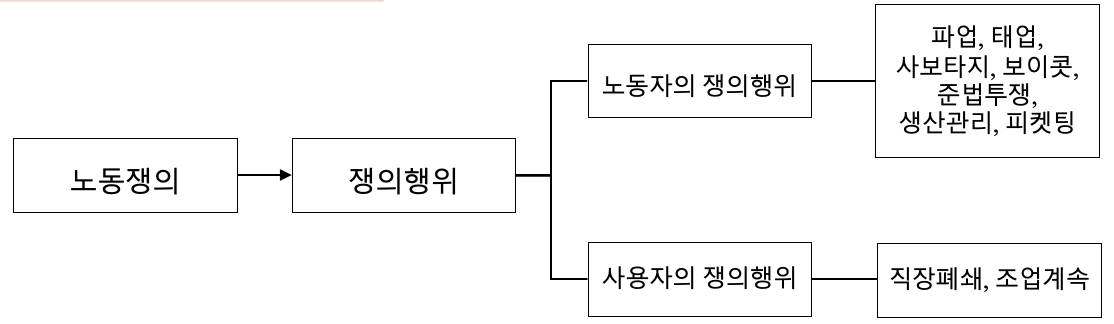
\includegraphics[width=.8\textwidth]{pic/노동쟁의도식.png}
        \caption{노동쟁의}
    \end{figure}
\end{frame}

\section{노사갈등의 개념}
\subsection{노사갈등에 대한 세 가지 시각}

\begin{frame}{일원론 입장}
    \begin{itemize}[<+->]
        \item 기업 내에서 노사간의 이해관계가 일치하기 때문에 노사간의 갈등이 존재하지 않는 것으로 보는 시각
        \item 기업 내에서 노사간의 이해관계가 완전히 일치하기 때문에 서로간의 갈등이 생기는 것은 경영자의 그릇된 경영방식에서 기인 
        \begin{itemize}[<+->]
            \item 노조의 존재이유와 노사갈등을 부정하는 시각
        \end{itemize}
        \item 경영자가 경영을 잘 하면 노사 갈등 발생 안할 것이라고 봄. 
        \begin{itemize}[<+->]
            \item 그러나 체계적이고 치밀한 경영을 하는 대기업에서 노조의 발생비율이 왜 높은지 설명하는데 한계
        \end{itemize}
    \end{itemize}
\end{frame}

\begin{frame}{급진적 입장}
    \begin{itemize}[<+->]
        \item 노사간의 갈등이 자본주의 사회에서 피할 수 없는 것으로 노사간의 갈등은 갈수록 더욱 격화되는 것으로 보는 시각
        \item 노사갈등을 해결하는 유일한 방법은 무산자계급의 혁명을 통하여 생산수단을 공유하는 공산주의체제로 전환하는 것 
        \begin{itemize}[<+->]
            \item 자본주의 사회와 사용자의 존재 가치를 인정하지 않는 시각
        \end{itemize}
        \item 단, 이 입장은 자본주의의 발달에도 불구하고 노사간의 갈등이 혁명으로 연결되지 않는 현실을 설명 못함
    \end{itemize}
\end{frame}

\begin{frame}{다원론 입장}
    \begin{itemize}[<+->]
        \item 한 기업 내에 노사 등 서로 다른 이해관계를 가진 집단이 존재하는 것을 인정하고 갈등은 필연적인 것으로 보는 시각
        \item 자본주의 사회에서 노사갈등은 필연적이나 가진 자와 못 가진 자간의 긴장이 간헐적으로 해소되어 혁명을 피할 수 있다고 주장 
        \begin{itemize}[<+->]
            \item 단체교섭이나 파업을 통해 노사간의 갈등이 해소되어 노동자의 불만이 해소되고 자본주의를 더욱 공고하게 만드는 효과가 있음
        \end{itemize}
        \item 노동조합의 존재와 파업의 존재가 오히려 자본주의 제도에 긍정적 효과를 준다고 주장
    \end{itemize}
\end{frame}

\begin{frame}[allowframebreaks]{노사갈등의 기본성격: 다원론 입장}
    \begin{itemize}[<+->]
        \item 노사갈등의 불가피성: 노사 당사자가 이성적이고 긍정적 사고를 가져도 노사갈등은 불가피
        \begin{itemize}[<+->]
            \item 노사 당사자의 무한 욕구와 이를 충족시킬 자원의 한정으로 분배의 만족을 이끌어내기 어려움
            \item 고용인과 노동자의 이해관계의 차이는 항상 존재
            \item 적정 분배방식이 수립되어도 원가상승, 제도변화, 소비자 구매패턴 변화 등 새로운 변수의 등장으로 분배방식을 재수립하여야 하는 역동성
            \item 노조와 기업조직은 태생적으로 상반된 목적을 갖고 있어 갈등은 나타날 수 밖에 없음 
        \end{itemize}
        \item 노사갈등의 다양성: 갈등을 겪는 개인이나 집단은 파업, 보이콧, 태업, 고충제기 등은 물론 이직, 결근 등을 표출하게 됨. 이직이나 결근 등은 침묵 파업 (silent strike)이라고 함
        \item 노사갈등의 수용가능: 노사갈등이 표출되면 당사자들이 많은 노력을 하게 되고 결국 분쟁이 해결되고 긴장감이 줄어 들어 자본주의체제가 더욱 공고해지는 효과. 다만, 과도하고 습관적이거나 병적인 갈등은 바람직하지 않음
    \end{itemize}
\end{frame}

\section{노동자의 쟁의행위}
\subsection{파업}%

\begin{frame}{파업의 정의}
    \begin{block}{파업}
        노사간의 주장의 불일치가 원인이 되어 노동조합이나 노동자집단의 주도하에 노동력을 생산수단과의 결합상태에서 분리시키고 사용자의 노동력에 대한 지휘·명령으로부터 노동자를 벗어나게 하는 상태
    \end{block}
\end{frame}

\begin{frame}[allowframebreaks]{파업의 분류}
    \begin{enumerate}[<+->]
        \item 의사결정 구성내용에 따른 분류
        \begin{itemize}[<+->]
            \item 계산적 파업 (rational strike): 상황에 대한 정확한 이해와 목적지향적인 행동에 근거하여 수행되는 파업
            \item 착오적 파업 (nonrational strike): 상대방의 의도나 행위 오해, 파업 결과를 잘못 추정, 부정확한 정보 등으로 발생 파업
            \item 충동적 파업 (irrational strike): 노조의 조직·지휘가 이루어지지 않거나, 방향성·목적성 없이 수행되는 충동적 파업
        \end{itemize}
    \framebreak\relax
        \item 조직상 분류: 노조의 조직 및 지시 여하에 따라 
        \begin{itemize}[<+->]
            \item 조합원파업: 노동조합의 조작 하에서 이루어지는 파업, 조직파업
            \item 비노조원파업: 노조의 규약 또는 지시에 위반하는 파업, 비조직파업
            \begin{itemize}[<+->]
                \item wild-cat strike: 노동조합 지도부의 승인을 받지 않고 소수의 조합원들에 의하여 행해지는 파업
            \end{itemize}
        \end{itemize}
        \item 참가범위에 따른 분류
        \begin{itemize}[<+->]
            \item 전면파업: 일정산업 또는 일정기업의 모든 조직 노동자가 파업에 참가
            \item 부분파업: 일부만이 파업에 참가
            \item 총파업 (general strike, 제네스트): 전국적으로 전 사업에 걸쳐서 행하여지는 파업
        \end{itemize}
    \framebreak\relax
        \item 쟁의행위의 선후에 따른 분류
        \begin{itemize}[<+->]
            \item 공격적 파업: 파업이 사용자의 직장폐쇄보다 선제적으로 행해지는 파업
            \item 방어적 파업: 직장폐쇄가 있은 다음에 행해지는 파업
        \end{itemize}
        \item 투쟁목적상 분류
        \begin{itemize}[<+->]
            \item 투쟁파업: 사용자의 주장을 꺾고 노동조합의 주장을 관철하려는 목적을 가진 파업
            \item 시위파업: 사용자에 대한 직접적인 투쟁목적이 없을 때 파업
            \item 경제파업: 임금 등 근로조건에 관한 자신의 주장을 관철하여 단체협약을 체결시키기 위한 파업
            \item 부당노동행위파업: 사용자의 단체협약 위반을 시정할 목적으로 행하는 파업 
        \end{itemize}
    \framebreak\relax
        \item 독자성 유무에 따른 분류
        \begin{itemize}[<+->]
            \item 자조적 파업: 파업을 수행하는 노동자들이 스스로의 주장을 관철하려고 할 때의 파업
            \item 동정 (연대)파업: 다른 파업의 지원을 목적으로 하는 파업.\ \textbf{노동법상의 파업이 아님}
        \end{itemize}
        \item 기한에 따른 분류
        \begin{itemize}[<+->]
            \item 무기한파업: 기한을 정하지 않은 파업
            \item 시한파업: 일정한 파업기간이 정해져 있는 파업
            \item 파상파업: 시한파업이 반복되어서 파상적으로 행해질 때의 파업
        \end{itemize}
    \end{enumerate}
\end{frame}

\subsection{태업 및 사보타지}

\begin{frame}{태업}
    \begin{block}{태업 (soldering)} 
        피고용인들이 단결해서 의식적으로 작업능률을 저하시키는 쟁의행위
    \end{block}
    \begin{itemize}[<+->]
        \item 방법: 생산작업의 속도 저하, 생산품의 양적 감소 초래, 고의적인 불량품 생산, 서비스의 질 하락 및 사용자 비난 등
        \item 파업과의 차이
        \begin{itemize}[<+->]
            \item 파업: 노동력을 생산수단과의 결합상태에서 분리. 사용자의 노동력에 대한 지휘·명령으로부터 완전히 벗어나게 하는 것
            \item 태업 또는 사보타지: 사용자의 지휘·명령을 그대로 따르지 않게 함
        \end{itemize}
    \end{itemize}
\end{frame}

\begin{frame}{사보타지}
    \framebreak\relax
    \begin{block}{사보타지 (sabotage)}
        생산 또는 사무를 방해하는 행위 및 의식적인 생산설비 파괴행위
    \end{block}
        \begin{itemize}[<+->]
            \item 소극적 사보타지 (passive sabotage): 생산 또는 사무를 방해하는 행위
            \item 적극적 사보타지 (active sabotage): 의식적으로 생산설비를 파괴하는 행위로 \textbf{노동법상 금지}
        \end{itemize}
\end{frame}

\subsection{준법투쟁}
\begin{frame}{준법투쟁}
    \begin{block}{준법투쟁 (work to rule)}
        권리·의무를 가진 피고용인들이 그들의 주장을 관철하기 위하여 법 규정을 엄격히 준수 또는 법률에 정한 피고용인의 권리를 동시에 집단적으로 행사함으로써 사용자의 업무 저해 행위
    \end{block}
    \begin{itemize}[<+->]
        \item 당해 규정을 객관적으로 요구하는 수준 이상으로 준수하여 작업의 능률을 저하시켜 사용자에게 압력수단으로 활용
        \item 준법투쟁의 예
        \begin{itemize}[<+->]
            \item 지하철 열차 운행 전, 규정에 정해진 모든 정비절차를 일시에 수행하여 운행 지연
            \item 관행화되어 있는 연장근로의 집단적 거부
            \item 연차·월차·병가 등의 집단적 사용 요구
        \end{itemize}
    \end{itemize}
\end{frame}

\subsection{보이콧}
\begin{frame}[allowframebreaks]{보이콧}
    \begin{block}{보이콧 (boycott)} 
        사용자 또는 그와 거래관계에 있는 제3자의 제품의 구입, 기타 시설의 이용을 거절한다던가, 사용자 또는 그와 거래관계에 있는 제3자와의 근로계약의 체결을 거절할 것을 요구하는 행위
    \end{block}
    \begin{itemize}[<+->]
        \item 쟁의행위 효과를 높이기 위해 부수적인 수단으로 행하여지며 대체로 미국에서 일반적임
    \end{itemize}
    \framebreak\relax
    \begin{itemize}[<+->]
        \item 일차적 보이콧 (primary boycott): 소비자가 사용자의 제품의 구매 또는 시설의 이용을 거부하게 함으로써 압력을 가는 행위 
        \begin{itemize}[<+->]
            \item 폭력적인 행위를 수반하지 않는 한 정당성 인정
        \end{itemize}
    \item 이차적 보이콧 (secondary boycott): 거래관계에 있는 제3자에게 사용자와의 거래를 단절할 것을 요구, 노동조합의 요구에 응하지 않을 경우 제품의 구입이나 시설의 이용, 또는 노동력의 공급을 중단하겠다는 압력을 가는 행위 
    \end{itemize}
\end{frame}

\subsection{생산관리}
\begin{frame}[allowframebreaks]{생산관리}
    \begin{block}{생산관리}
        노동자들이 단결하여 사용자의 지휘·명령을 거부하면서 사업장 또는 공장을 점거하고 조합간부의 지휘 하에 노무를 제공하는 투쟁행위
    \end{block}
    \begin{itemize}[<+->]
        \item 종전의 경영방침을 따르면서 다만 노동자들이 직접 경영을 하되 수익은 회사를 위하여 보관하고 임금을 종래대로 지급하는 방식
        \begin{itemize}[<+->]
            \item 이상형 생산관리  
        \end{itemize}
    \framebreak\relax
    \item 회사자재를 마음대로 처분하거나 회사의 수익금을 일방적으로 인상한 임금에 충당하는 경우
    \item 단순한 노무거부를 넘어 공장·사업장 또는 설비 등을 점유하여 사용자의 지휘·명령을 배제하기 때문에 사용자의 소유권과 기업경영권을 침해하는 것 
    \item 원칙적으로 \textbf{부당한 쟁의행위}임
    \end{itemize}
\end{frame}

\subsection{기타 행위}
\begin{frame}{피켓팅}
    \begin{block}{피켓팅 (picketing)}
        파업을 효과적으로 수행하기 위하여 근로희망자 (파업 비참가자)들의 사업장 또는 공장의 출입을 저지하고 파업참여에 협력할 것을 요구하는 행위     
    \end{block}
\end{frame}

\begin{frame}{부수적 쟁의 수단}
    \begin{itemize}[<+->]
        \item 문서배포 등: 조합원의 쟁의행위 참가·설득을 위해 전단 및 벽보 등의 배포·부착·현수막의 게시
        \begin{itemize}[<+->]
            \item 사용자의 강제철거 및 금지명령은 위법으로 사용자의 부당노동행위
            \item 단, 표현 내용이 신용 및 명예 등의 훼손, 업무에 대한 구체적인 지장을 줄 경우 형사상 책임 부과
        \end{itemize}
    \item 리본·완장 등: 항의 표시 및 단결 고취를 위해 리본·완장·머리띠·어깨띠 등을 부착하는 행위
        \begin{itemize}[<+->]
            \item 통상적 업무에 지장을 초래하지 않으므로 위법이라고 하기 어려움
            \item 단, 종사업무의 성질에 따라 노동력의 불완전한 제공이 될 경우 신중한 고려 필요
        \end{itemize}
    \item 직장점거: 파업시 사태에 대한 기민한 대처·단결력 확보 등을 위해 사업장에 체류하는 행위
        \begin{itemize}[<+->]
            \item 부수적인 쟁의행위로 연좌 또는 농성을 하는 연좌파업의 모습을 띠기도 함
        \end{itemize}
    \end{itemize}
\end{frame}

\section{사용자측의 대항행위}

\begin{frame}{직장폐쇄 (lockout)}
    \begin{itemize}[<+->]
        \item 사용자가 자가의 주장을 관철하기 위하여 노동자 집단에 대하여 생산수단에의 접근을 차단하고 노동자의 노동력 수령을 조직적·집단적·일시적으로 거부하는 행위 
        \item 따라서 경영상의 사정으로 인한 휴업이나 사업장 폐쇄, 출근정지처분은 직장폐쇄가 아님
        \item 직장폐쇄가 종료되면 노무의 수령이 거부되었던 노동자들을 다시 취업시킨다는 전제로
    \end{itemize}
\end{frame}

\begin{frame}{조업계속}
    \begin{itemize}[<+->]
        \item 노동조합의 동맹파업 시 노동조합원 이외의 노동자 또는 노동조합원 중 근로희망자를 사용해서 조업을 하는 행위
        \item 조업계속을 통해 조업 참가자에게 임금이 지급되고 비참가자는 임금이 지급되지 않아 결국 노동조합의 결속력을 와해 시키려는 방법의 일환
    \end{itemize}
\end{frame}

\section{노동쟁의의 의사결정}

\begin{frame}[allowframebreaks]{의사결정시 고려사항}
    \begin{itemize}[<+->]
        \item 파업 실시여부는 신중하게 결정하여야 
        \begin{itemize}[<+->]
            \item ∵ 노사는 물론 국가 전체에 엄청난 악영향을 줄 수 있기 때문에
        \end{itemize}
    \end{itemize}
    \begin{enumerate}[<+->]
            \item 사용자측: 파업발생을 대비하여 검토할 사항
        \begin{itemize}[<+->]
            \item 파업으로 인한 손익을 사전에 정확하게 산출해야
            \item 파업기간 동안 조업의 지속여부
            \item 파업 가능성이 높아지면 고객에 대한 파업 가능성 고지 및 대응방안 (예: 본사제품 추가 구매, 대체품 매입 알선 등) 강구
    \framebreak\relax
        \end{itemize}
        \item 노조측: 파업에 돌입하기 전에 파업으로 인한 득실 평가 필요
        \begin{itemize}[<+->]
            \item 파업에 얼마나 많은 조합원이 동참하여 사용자의 조업계속을 무산시킬 수 있을 것인가?
            \item 파업이 장기화될 경우 파업기금에서 조합원들을 지속적으로 지원할 수 있는가?
            \item 노조의 요구사항이 사용자의 지불능력 범위 내에 있는가?
            \item 정부나 여론의 향배 분석
        \end{itemize}
    \end{enumerate}
\end{frame}

\section{한국의 노동쟁의 법규}%

\begin{frame}[allowframebreaks]{쟁의행위의 목적}
    \begin{block}{쟁의행위}
        파업·태업·직장폐쇄 기타 노동관계 당사자가 그 주장을 관철할 목적으로 행하는 행위와 이에 대항하는 행위로서 업무의 정상적인 운영을 저해하는 행위
    \end{block}
    \begin{itemize}[<+->]
        \item 목적: 단체교섭에 의해 타결하려던 임금·노동시간·복지·해고 기타 근로조건의 유지·개선
        \item 한국의 노동법규에서는 권리분쟁과 이익분쟁 중 이익분쟁만 적법한 쟁의로 인정
        \begin{itemize}[<+->]
            \item 권리분쟁에 의한 쟁의행위나 동정파업, 정치적 파업 등은 적법한 쟁의행위가 아님
        \end{itemize}
        \item  권리분쟁: 법령, 단체협약, 취업규칙 등에 의하여 이미 확정된 권리에 관한 노사간 해석,적용,준수 등을 둘러싼 분쟁 
        \begin{itemize}[<+->]
            \item 체불임금 청산, 해고자 복직, 단체협약 이행, 부당노동행위 구제 등이 이에 해당됨.
        \end{itemize}
        \item 이익분쟁: 근로조건의 기준에 관한 권리의 형성,유지,변경 등을 둘러싼 분쟁
        \begin{itemize}[<+->]
            \item 임금인상이나 단협 갱신,체결 등
        \end{itemize}
    \end{itemize}
\end{frame}

\begin{frame}[allowframebreaks]{쟁의행위의 절차}
    \begin{itemize}[<+->]
        \item 적법한 쟁의행위의 기준 준수 필요: 형사상·민사상의 면책이 부여
        \begin{itemize}[<+->]
            \item 쟁의의 내용이 노동조합과 사용자 사이의 문제, 즉 경제적 지위의 향상에 관한 것
            \item 정치적 문제를 이유로 한 파업은 불법
            \item 사회적 통념에 비추어 부당하거나 불가능한 또는 과대한 요구를 내세운 쟁의는 아니어야 함
            \item 노동조합 조합원의 직접·비밀·무기명 투표에 의한 조합원 재적 과반수의 찬성을 받아야 함
        \end{itemize}
    \item 조정전치주의 채택: 노동조합이 쟁의행위를 하기 전에 반드시 노동위원회의 조정을 받아야 함
    \item 쟁의행위 사전신고의 의무 부과: 노동부 장관과 관할 노동위원회에 쟁의행위의 일시, 장소, 참가인원 및 그 방법을 신고하여야 한다고 규정
    \end{itemize}
\end{frame}

\begin{frame}[allowframebreaks]{피고용인의 쟁의행위와 민형사상 면책}
    \begin{itemize}[<+->]
        \item 『노동조합 및 노동관계조정법』에서 정당한 쟁의행위에 대한 민형사상의 면책 규정
        \begin{itemize}[<+->]
            \item 형사상 면책: 노동자가 근로조건을 유지·개선하기 위하여 단체교섭, 기타의 행위를 함에 있어서 그 행위가 정당성을 가지는 한 이를 처벌하지 않음
            \item 민사상 면책: 사용자는 정당한 쟁의행위로 인한 손해를 받은 경우 노조 및 근로자에게 그 배상을 청구할 수 없음
        \end{itemize}
        \item 단, 노동조합과 근로자가 행하는 불법파업에 대해서는 민형사상의 책임을 피할 수 없음.
        \item 손해배상 및 가압류: 노동조합의 불법 또는 위법이나 고의 과실 등에 의해 사업주가 손해를 봤을 때 해당 노동조합 또는 노조원을 상대로 손해배상을 청구하는 행위. 
        \begin{itemize}[<+->]
            \item 더불어 그 청구 전 우선하여 상대방 재산에 대해 은닉이나 도피, 감소 등을 방지하기 위해 가압류하는 행위를 손배가압류라 함.
        \end{itemize}
        \item `노란봉투법': 노동조합 및 노동관계 조정법 제3조 (손해배상 청구의 제한)
        \begin{itemize}[<+->]
            \item 사용자는 이 법에 의한 단체교섭 또는 쟁의행위로 인하여 손해를 입은 경우에 노동조합 또는 근로자에 대하여 그 배상을 청구할 수 없다.
        \end{itemize}
    \end{itemize}
\end{frame}

\begin{frame}[allowframebreaks]{사용자의 대항행위 관련 법규}
    \begin{enumerate}[<+->]
        \item 직장폐쇄: 사용자는 노동조합이 쟁의행위를 개시한 이후에만 직장폐쇄를 할 수 있음
        \begin{itemize}[<+->]
            \item 수동적·방어적인 직장폐쇄만을 사용자의 정당한 쟁의행위로 인정
        \end{itemize}
        \item 조업계속과 대체근로: 노조의 쟁의행위 시 파업불참자와 비노조원을 사용하여 조업계속 가능.
        \begin{itemize}[<+->]
            \item 쟁의행위 중단·업무 수행을 위해 신규로 노동자 채용은 금지
        \end{itemize}
    \end{enumerate}
    \framebreak\relax
    \begin{itemize}[<+->]
        \item 조업계속: 사용자는 노조의 쟁의행위 시 파업불참자와 비노조원을 사용하여 조업 계속 가능
        \item 노조의 쟁의행위 시 사업과 관계없는 자를 채용 또는 대체할 수 없음
        \item 단, 노동쟁의가 필수공익사업에서 발생한 경우 공익보호를 위해, 파업인원의 절반까지 신규인력이나 외부인력을 일시로 고용하거나 다른 회사에 외주를 주어 조업을 계속하는 것은 허용
    \end{itemize}
\end{frame}

\begin{frame}{쟁의행위중의 임금지급}
    \begin{itemize}[<+->]
        \item 쟁의행위기간 중의 임금지급 금지: 무노동·무임금 (no work, no pay)의 원칙
        \begin{itemize}[<+->]
            \item 사용자는 쟁의행위에 참가하여 근로를 제공하지 않은 근로자에 대해 그 기간 중의 임금을 지급할 의무가 없음
            \item 노조는 쟁의행위 기간에 대한 임금의 지급을 요구하거나 이를 관철할 목적으로 쟁의행위를 하여서는 아니 됨
        \end{itemize}
    \item 단, 쟁의행위 중 파업에 참가하지 않고 실질적으로 근로한 근로자에 대해서는 당연히 임금을 지급하여야 함
    \end{itemize}
\end{frame}

\section{한국의 노동쟁의 현황}%

\begin{frame}{1987년 이전: 정치적위기와 파업}
    \begin{figure}
        \centering
        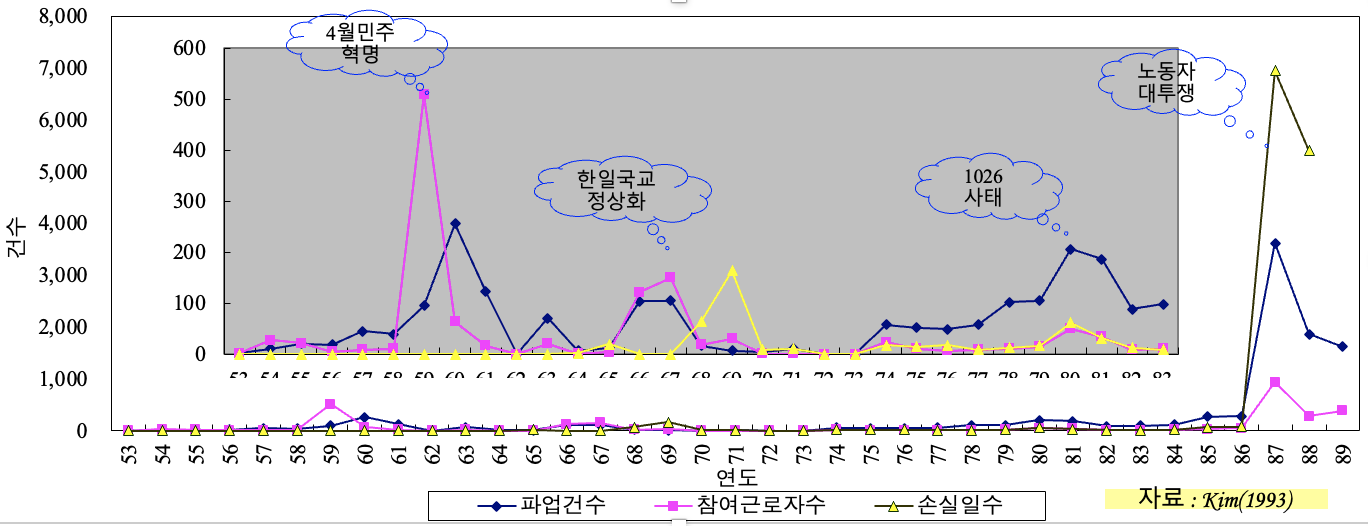
\includegraphics[width=.7\textwidth]{pic/87년이전파업.png}
        \caption{1987년 이전의 파업추이}
    \end{figure}
    \begin{itemize}[<+->]
        \item 1987년까지 노동법은 파업을 억제하기 위해 파업요건을 까다롭게 규정 
        \item 정부통제력이 약화되는 시기에 파업이 집중적으로 발생. 
    \end{itemize}
\end{frame}

\begin{frame}{1987년 이후 노동쟁의 특징}
    \begin{itemize}[<+->]
        \item 1987년을 정점으로 차츰 감소하다가 1997년 경제위기 이후 다소 증가, 2004년 다시 감소, 2017년 다시 상승세. 1987년 이후 파업발생은 완만한 사이클을 보이면서 하락과 상승 반복 
        \item 발생원인을 보면 대체로 임금보다는 근로조건과 고용 이슈가 중요
        \item 업종별로 보면 제조업이 전체 파업의 과반 차지
    \end{itemize}
\end{frame}


%------------------------------------------------
\end{document}
%------------------------------------------------
